\chapter{Introducción}
\label{chap:introduction}
\textit{En la presente sección se hablará a grandes rasgos el tema de interés de la tesis
y las técnicas para estudiarlo.}
\vfill
\minitoc
\newpage

\section{Motivación del trabajo}
\label{ch1-why}
Este trabajo tiene como finalidad entender las propiedades de los semiconductores \mbox{CdTe (001)} y \mbox{Hg$_{0.18}$Cd$_{0.82}$Te (001)}, siendo sometidos a un estrés o tensión causada sobre su superficie. Esto con la finalidad de establecer un \textit{estándar} para comprender las propiedades de los materiales llamados \textit{aislantes topológicos}, aunque ninguno de los materiales estudiados están en este grupo, sus compuestos y heteroestructuras sí presentan algunas propiedades topológicas. Además, se realizó la implementación electrónica y de programas de control para obtener los espectros de Reflectancia Diferencial, en el monocromador HR60.

\section{Aislantes Topológicos}
\label{ch1-ti}
La forma mas simple de describir un aislante topológico es como un aislante cuya frontera con el vacío siempre permanece metálica. Para que un aislante topológico se forme, la interacción espín-orbita debe ser fuerte y modificar significativamente la estructura electrónica. Esto sugiere que los semiconductores de brecha fundamental muy pequeña sean muy adecuados para configurar aislantes topológicos. Dentro de los materiales con fases topológicas podemos mencionar la aleación \mbox{Bi$_{x}$Sb$_{1-x}$} y el semimetal HgTe\cite{Konig2007, Moore2010}. Se caracterizan por estados exóticos metálicos, en las cuales los electrones viajan insensibles a las colisiones producidas por las impurezas\cite{Moore2010, Konig2007}.

La idea sobre los aislantes topológicos surgió del trabajo del efecto Hall Cuántico. Este efecto que se presenta en estructuras semiconductoras de dos dimensiones bajo un campo magnético externo\cite{Klitzing1980}. Una traza de este efecto debe de observarse aun sin la presencia de un campo magnético externo considerando que en un semiconductor los electrones al moverse dentro del mismo, sentirán un campo magnético efectivo producido por los núcleos positivos del cristal (el llamado acople espín-orbita o SOC, por sus siglas en ingles).

Las interfaces metal/semiconductor de materiales con un fuerte SOC presentan el \textit{efecto Rashba} que aunque no son aislantes topológicos como tal, presentan algunos fenómenos de los mismos, como la formación de corrientes Hall en su superficie\cite{Lin2014, Bihlmayer2015}.

\section{Diagrama de bandas de CdTe y HgTe}
\label{ch1-band-diagram}
El CdTe es un semiconductor directo cuya brecha fundamental a una temperatura de \mbox{300 K} es \mbox{E$_{g}$=1.44 eV} \cite{Kittel2004-yd, Chadi1972}. Se muestra en la Fig. \ref{fig:band_diagram} (a) el diagrama simplificado de bandas en el punto $ \Gamma $ del centro de la zona de Brillouin\cite{Chadi1972}. La banda de valencia de los huecos ligeros y pesados tiene una simetría $ \Gamma_{8} $ y está degenerada por $n=4$. La banda \textit{Split-off} es de simetría $ \Gamma_{7} $ y degeneración $n=2$. La banda de conducción, tiene una simetría  $ \Gamma_{6} $ y degeneración $n=2$. En la misma figura se muestra las bandas para HgTe\cite{Chadi1972}.

\begin{figure}[H]
    \centering
    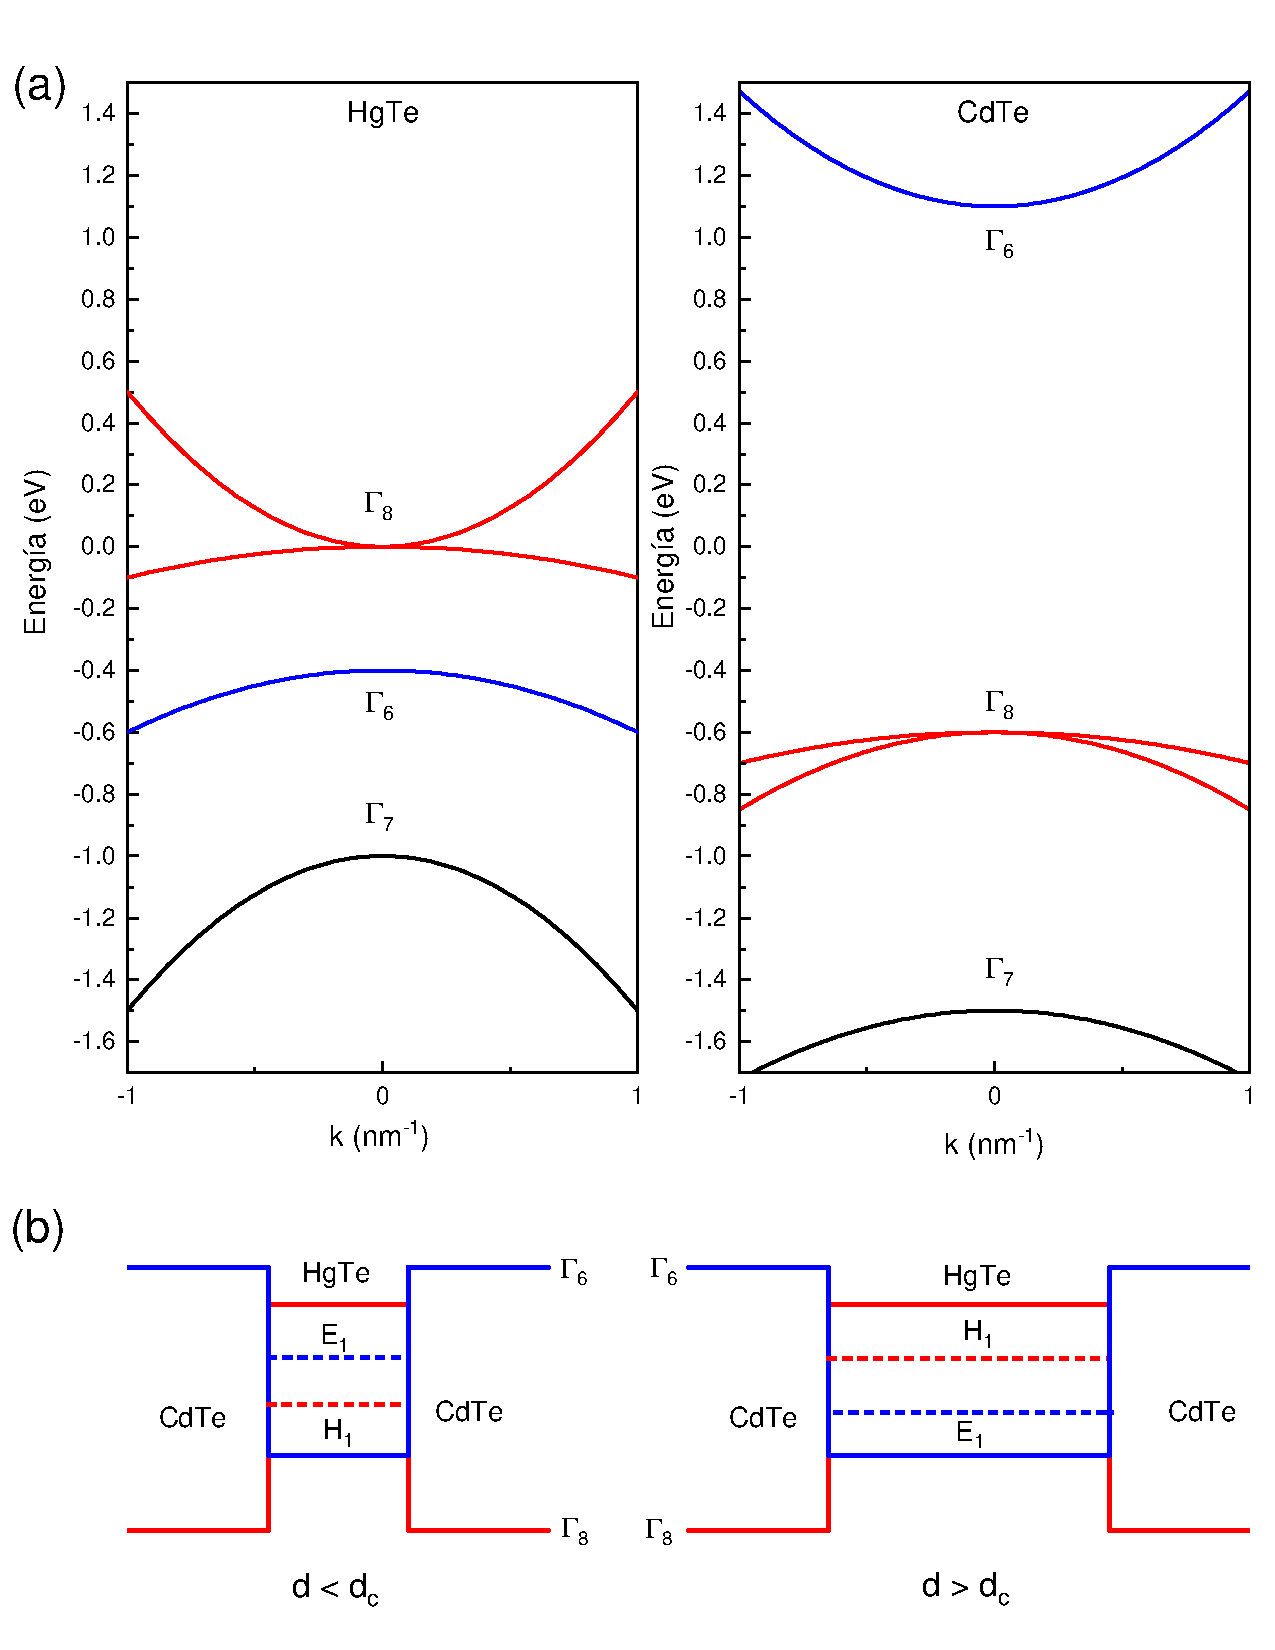
\includegraphics[width=0.7\textwidth]{figures/chap3/band_diagram.pdf}
        \caption{(a) Diagrama de bandas para los semiconductores CdTe y HgTe. (b) Diagrama de bandas para el pozo bidimensional CdTe/HgTe/CdTe para diferentes casos de $ d = d_{c} $\cite{Bernevig2006}.}
    \label{fig:band_diagram}
\end{figure}

Es importante notar, que el orden energético de las bandas  $ \Gamma_{6} $ y $ \Gamma_{8} $ no es el mismo para CdTe y HgTe. Mientras que para HgTe la energía de la banda $ \Gamma_{6} $  es menor que para la banda  $ \Gamma_{8} $, para el CdTe el orden de las bandas es el contrario.

Lo anterior tiene consecuencias muy importantes en el caso de las estructuras de pozos basados en CdTe/HgTe. Para comprender esta importancia se muestra en la \ref{fig:band_diagram} (b) un diagrama de las bandas de una estructura de pozos bidimensionales de CdTe/HgTe/CdTe\cite{Bernevig2006}.
Para un cierto espesor \textit{d} del HgTe por debajo de un espesor critico $ d_{c} $, siendo definido cuando se cumple la condición $ E_{1} = H_{1} $. Los niveles de los estados de los portadores $ E_{1} $ y $ H_{1} $ atrapados en el pozo tiene valores como los que se muestran en \ref{fig:band_diagram} (b), es decir $ E_{1}>H_{1} $. 
Al incrementar $d$ por encima del valor crítico $ d_{c} $, las energías de los portadores evolucionan hasta llegar a la relación $ E_{1}<H_{1} $ en sus energías, es decir se produce una \textit{inversión} de las energías.

Este punto de inversión de las energías es también el punto de conversión entre un aislante convencional y un aislante topológico. Es decir, para $ d $ $ > $ $ d_{c} $ el sistema presenta una fase topológica \cite{Bernevig2006}.
Otra forma de manipular las bandas de energía en el HgTe y lograr fases topológicas, es por medio de la aplicación de una tensión. La tensión puede generarse a través del sustrato de CdTe sobre el que se crece el HgTe o aplicando la tensión externamente. En ambos casos, la degeneración de la banda $ \Gamma_{8} $ es removida eliminando el carácter de semimetal del HgTe y produciendo una fase de aislante topológico \cite{Brne2011, Wu2014}. 

\section{Técnicas Ópticas de Caracterización}
\label{ch1-opt-charac-tech}
Las técnicas ópticas de caracterización, utilizan la luz como sonda para obtener diferentes propiedades de los materiales, que van desde su morfología y estructura molecular, hasta de carácter electrónico, de forma segura, ya que son técnicas no destructivas que pueden aplicarse tanto \textit{in-situ} o \textit{ex-situ}. En el presente trabajo, se busca entender las propiedades de los materiales de interés antes mencionados, por medio de las siguientes técnicas.

\begin{itemize}
    \item Reflectancia diferencial espectroscópica (RDS). Esta técnica es sensible al rompimiento 
    de simetría. En semiconductores o estructuras cubicas la RDS da información del estado de la superficie o de las interfaces. Esta técnica es una herramienta potencial para el estudio de las interfaces aislante/metal que se produce en los aislantes topológicos.

    \item Espectroscopia Raman. En este trabajo, se utilizará para caracterizar las interfaces 
    metal/semiconductor, ya que esta técnica sondea la estructura del material utilizando un haz de luz 
    monocromático. Además de darnos una idea del estrés relativo al que esta sometido el material, siendo 
    un parámetro importante para el estudio de los aislantes topológicos.

    \item Microscopia de Fuerza Atómica (AFM) y Microscopia Óptica de Campo Cercano 
    (NSOM). La unión de ambas técnicas nos da una idea de la morfología por medio de AFM, utilizando las fuerzas atractivas y repulsivas en la interaccion sistema/muestra y la respuesta óptica del material por medio de NSOM, por lo que podemos caracterizar superficies y complementar las otras técnicas.
\end{itemize}

El conjunto de estas técnicas nos permite caracterizar la interfaz metal/semiconductor, en sus tres zonas de interés, la morfología y respuesta óptica de la superficie; las anisotropías en la interfaz y la tensión o daños causados al substrato.